
\subsection{CIFAR10}
\label{sub:cifar_appx}

This section provides more extensive results for the experiments on CIFAR10 from Section~\ref{sub:exp_smalldata}.
In particular, Table~\ref{tab:smalldata_ext} shows additional experiments on larger subsets of size 5\.000,
as well as more methods, including different geometries (see Appendix~\ref{sec:non_euclidian_appx}).
The table also reports results obtained when using a smaller validation set of size 1\,000.
The full hyper-parameter grid is given in Table~\ref{tab:smalldata_param_grid}.

In order to assess the statistical significance of our results,
we repeated the experiments on 10 new random choices of subsets, using the hyperparameters selected
on the original subset from Table~\ref{tab:smalldata_ext} (except for learning rate, which is selected according to a different validation set for each subset).
We then compared pairs of methods using a paired t-test, with p-values shown in Table~\ref{tab:t_test}.
In particular, the results strengthen some of our findings, for instance, that $\|\nabla f \|^2$
should be preferred to the gradient penalty on the loss when there is no data augmentation,
and that combined upper+lower bound approaches tend to outperform the individual upper or lower
bound strategies.


\begin{table}[h]
\caption{Regularization on CIFAR10 with 1\,000 or 5\,000 examples for VGG-11 and ResNet-18.
Extended version of Table~\ref{tab:smalldata}.
Each entry shows the test accuracy with/without data augmentation when all hyper-parameters are optimized on a validation set of size 10\,000 (a) or 1\,000 (b),
and for the epoch with highest validation accuracy,
evaluating every 10 epochs (similar to early stopping).}
\centering
\vspace{0.2cm}
\label{tab:smalldata_ext}
(a) 10k examples in validation set

% python print_table.py --full
\begin{tabular}{ | l | c | c | c | c |  }
\hline
Method & 1k VGG-11 & 1k ResNet-18 & 5k VGG-11 & 5k ResNet-18 \\ \hline
\hline
No weight decay & 50.70 / 43.75 & 45.23 / 37.12 & 72.49 / 58.35 & 72.72 / 54.12 \\
Weight decay & 51.32 / 43.95 & 44.85 / 37.09 & 72.80 / 58.56 & 73.06 / 53.33 \\
SN penalty (PI) & 54.64 / 45.06 & 47.01 / 39.63 & 74.03 / 62.45 & 74.79 / 54.04 \\
SN penalty (SVD) & 53.44 / 46.06 & 47.26 / 37.94 & 74.53 / 62.93 & 75.59 / 54.98 \\
SN projection & 54.14 / \textbf{\color{darkgray}46.70} & 47.12 / 37.28 & 75.14 / 63.81 & 76.23 / 55.60 \\
VAT & 50.88 / 43.36 & 47.47 / 42.82 & 72.91 / 58.78 & 71.56 / 55.93 \\
PGD-$\ell_2$ & 51.25 / 44.40 & 45.80 / 41.87 & 73.18 / 58.98 & 72.53 / 55.92 \\
PGD-$\ell_\infty$ & 51.17 / 43.07 & 45.31 / 39.66 & 73.05 / 57.82 & 72.75 / 55.14 \\
grad-$\ell_2$ & \textbf{\color{darkgray}55.19} / 43.88 & \textbf{49.30} / \textbf{\color{darkgray}44.65} & \textbf{75.38} / 59.20 & 75.22 / 55.36 \\
grad-$\ell_1$ & 54.88 / 44.74 & \textbf{\color{darkgray}49.06} / 42.63 & \textbf{\color{darkgray}75.25} / 59.39 & 74.48 / 56.19 \\
\hline
$\|f\|_\delta^2$ penalty & 51.41 / 45.07 & 48.73 / 43.72 & 72.98 / 61.45 & 72.78 / 56.50 \\
$\|\nabla f\|^2$ penalty & 54.80 / 46.37 & \textbf{\color{darkgray}48.99} / \textbf{44.97} & 73.90 / 60.17 & 73.83 / \textbf{\color{darkgray}57.92} \\
PGD-$\ell_2$ + SN proj & 54.19 / \textbf{\color{darkgray}46.66} & 47.47 / 41.25 & 74.61 / \textbf{64.50} & \textbf{\color{darkgray}77.19} / 57.43 \\
grad-$\ell_2$ + SN proj & \textbf{55.32} / \textbf{46.88} & 48.73 / 42.78 & 75.11 / 63.54 & \textbf{77.73} / 57.09 \\
$\|f\|_\delta^2$ + SN proj & 54.02 / \textbf{\color{darkgray}46.72} & 48.12 / 43.56 & 74.55 / \textbf{\color{darkgray}64.33} & 75.64 / \textbf{59.03} \\
$\|\nabla f\|^2$ + SN proj & \textbf{55.24} / \textbf{46.80} & \textbf{\color{darkgray}49.06} / \textbf{44.92} & 72.31 / 63.74 & 72.24 / 57.56 \\
\hline
\end{tabular}
\\
\vspace{0.2cm}
(b) 1k examples in validation set

% python print_table.py --full --small_val
\begin{tabular}{ | l | c | c | c | c |  }
\hline
Method & 1k VGG-11 & 1k ResNet-18 & 5k VGG-11 & 5k ResNet-18 \\ \hline
\hline
No weight decay & 51.32 / 43.42 & 45.00 / 37.00 & 72.64 / 57.88 & 72.71 / 53.80 \\
Weight decay & 51.04 / 43.42 & 44.66 / 36.77 & 72.68 / 57.59 & 72.25 / 54.16 \\
SN penalty (PI) & 54.60 / 44.20 & 46.39 / 38.86 & 72.99 / 62.49 & 74.72 / 53.65 \\
SN penalty (SVD) & 53.76 / 44.79 & 47.31 / 37.92 & 74.05 / 63.34 & 75.73 / 54.65 \\
SN projection & 52.86 / \textbf{\color{darkgray}46.49} & 47.05 / 37.28 & 74.18 / \textbf{\color{darkgray}63.70} & 75.91 / 54.43 \\
VAT & 50.90 / 43.99 & 47.35 / 42.91 & 72.95 / 57.64 & 71.91 / 55.22 \\
PGD-$\ell_2$ & 50.95 / 43.26 & 45.77 / 41.71 & 72.71 / 57.68 & 72.87 / 54.17 \\
PGD-$\ell_\infty$ & 51.16 / 43.16 & 45.67 / 39.77 & 73.64 / 58.02 & 72.99 / 53.95 \\
grad-$\ell_2$ & \textbf{55.40} / 43.57 & 47.86 / \textbf{\color{darkgray}44.65} & \textbf{75.44} / 58.33 & 74.83 / 55.43 \\
grad-$\ell_1$ & 54.53 / 43.04 & \textbf{\color{darkgray}48.75} / 42.21 & \textbf{\color{darkgray}75.28} / 58.19 & 74.28 / 54.02 \\
\hline
$\|f\|_M^2$ penalty & 51.00 / 44.67 & 48.57 / 44.30 & 72.76 / 60.55 & 72.75 / 56.49 \\
$\|\nabla f\|^2$ penalty & 54.68 / 46.10 & 48.53 / \textbf{45.21} & 73.83 / 60.36 & 73.30 / \textbf{\color{darkgray}57.46} \\
PGD-$\ell_2$ + SN proj & 53.85 / \textbf{46.79} & 46.48 / 40.95 & 74.79 / 63.37 & \textbf{\color{darkgray}76.28} / \textbf{\color{darkgray}57.43} \\
grad-$\ell_2$ + SN proj & \textbf{\color{darkgray}55.28} / 45.11 & 48.42 / 41.93 & 75.17 / 63.45 & \textbf{77.24} / 56.18 \\
$\|f\|_M^2$ + SN proj & 54.00 / 45.14 & 47.12 / 41.86 & 74.54 / \textbf{63.94} & 75.25 / \textbf{57.94} \\
$\|\nabla f\|^2$ + SN proj & \textbf{\color{darkgray}55.21} / 45.68 & \textbf{49.03} / 43.58 & 71.92 / 63.47 & 71.83 / 56.06 \\
\hline
\end{tabular}
\end{table}


\begin{table}[h]
\caption{Paired t-tests comparing pairs of methods, on 10 different random choices of subsets of CIFAR10.
Each cell shows the p-value of the corresponding test, both with (left) and without (right) data augmentation.
We only show p-values smaller than~$0.05$.
Hyperparameters are fixed to the ones obtained for the results in Table~\ref{tab:smalldata}
(selected on a different choice of subset), except for the learning rate which is tuned on
a separate validation set for each choice of subset.}
\centering
\label{tab:t_test}
\vspace{0.2cm}
% python print_significance_table.py --test_type ttest --optlr
\begin{tabular}{ | c | c c | c c | c c | c c |  }
\hline
Test & \multicolumn{2}{|c|}{1k VGG-11} & \multicolumn{2}{|c|}{1k ResNet-18} & \multicolumn{2}{|c|}{5k VGG-11} & \multicolumn{2}{|c|}{5k ResNet-18} \\ \hline
\hline
SN projection $\succ$ Weight decay & 1e-04 & 1e-03 & - & - & 3e-06 & 1e-08 & 9e-07 & 4e-04\\ \hline
grad-$\ell_2$ $\succ$ Weight decay & 4e-09 & - & 2e-04 & 5e-05 & 7e-08 & 1e-04 & 5e-06 & -\\ \hline
$\|\nabla f\|^2$ $\succ$ Weight decay & 1e-08 & 2e-07 & 1e-05 & 3e-07 & 3e-04 & 5e-07 & 7e-03 & 1e-06\\ \hline
$\|\nabla f\|^2$ $\succ$ grad-$\ell_2$ & - & 3e-08 & 2e-02 & 2e-06 & - & 6e-05 & - & 4e-05\\ \hline
grad-$\ell_2$ $\succ$ $\|\nabla f\|^2$ & 2e-02 & - & - & - & 2e-05 & - & 7e-04 & -\\ \hline
grad-$\ell_2$ + SN proj $\succ$ grad-$\ell_2$ & - & 9e-03 & - & - & - & 5e-07 & 9e-06 & 2e-04\\ \hline
$\|\nabla f\|^2$ + SN proj $\succ$ $\|\nabla f\|^2$ & - & - & - & 1e-02 & - & 2e-06 & - & -\\ \hline
\end{tabular}
\end{table}

\begin{table}[h]
\caption{List of hyper-parameters used for each method on CIFAR10.
For each method, we additionally consider a learning rate parameter in $[0.003 ; 0.01 ; 0.03 ; 0.1]$.
For combined penalties, the sets of hyperparameters are listed in the same order as in the first column
(\ie, the choices of constraint radius are given last).}
\centering
\small
\vspace{0.2cm}
\label{tab:smalldata_param_grid}
\begin{tabular}{ | l | c |  }
\hline
Method & Parameter grid \\ \hline
\hline
No weight decay &  -   \\ \hline
Weight decay &  $[0; 0.0001 ; 0.0002 ; 0.0004 ; 0.0008 ; 0.001 ; 0.002]$   \\ \hline
SN penalty (PI) &  $[0.001 ; 0.003 ; 0.01 ; 0.03 ; 0.1 ; 0.3]$ \\ \hline
SN penalty (SVD) &  $[0.001 ; 0.003 ; 0.01 ; 0.03 ; 0.1 ; 0.3]$  \\ \hline
SN projection &  $[0.5 ; 0.6 ; 0.8 ; 1.0 ; 1.2 ; 1.4]$  \\ \hline
$\|f\|_\delta^2$ penalty & $[0.001 ; 0.003 ; 0.01 ; 0.03 ; 0.1]$  \\ \hline
$\|\nabla f\|^2$ penalty & $[0.00003 ; 0.0001 ; 0.0003 ; 0.001 ; 0.003 ; 0.01 ; 0.03]$ \\ \hline
VAT & $[0.1 ; 0.3 ; 1.0 ; 3.0]$ \\ \hline
PGD-$\ell_2$ &  $[0.003 ; 0.01 ; 0.03 ; 0.1 ; 0.3 ; 1.0]$ \\ \hline
PGD-$\ell_\infty$ &  $[0.001 ; 0.003 ; 0.01 ; 0.03 ; 0.1 ; 0.3]$  \\ \hline
grad-$\ell_1$ &  $[0.0001 ; 0.0003 ; 0.001 ; 0.003 ; 0.01 ; 0.03]$  \\ \hline
grad-$\ell_2$ &  $[0.001 ; 0.003 ; 0.01 ; 0.03 ; 0.1 ; 0.3 ; 1.0 ; 3.0]$ \\ \hline
PGD-$\ell_2$ + SN projection &  $ [0.003 ; 0.01 ; 0.03 ; 0.1] \times [0.6 ; 1.0 ; 1.4]$   \\ \hline
grad-$\ell_2$ + SN projection & $ [0.003 ; 0.01 ; 0.03 ; 0.1] \times [0.6 ; 1.0 ; 1.4]$  \\ \hline
$\|f\|_\delta^2$ + SN projection & $ [0.003 ; 0.01 ; 0.03] \times [0.6 ; 1.0 ; 1.4]$    \\ \hline
$\|\nabla f\|^2$ + SN projection & $ [0.001 ; 0.01 ; 0.1] \times [0.6 ; 1.0 ; 1.4]$   \\ \hline
\end{tabular}
\end{table}

\subsection{Infinite MNIST}
\label{sub:imnist_appx}

We provide more extensive results for the Infinite MNIST dataset in Table~\ref{tab:imnist_ext},
in particular showing more regularization strategies, as well as results with or without
data augmentation, marked with~$(\ast)$.
As in the case of CIFAR10, we use SGD with momentum (fixed to 0.9) for 500 epochs,
with initial learning rates in~$[0.005; 0.05; 0.5]$, and divide the step-size by 2 every 40 epochs.
The full hyper-parameter grid is given in Table~\ref{tab:imnist_param_grid}.


As in the case of CIFAR10, we report statistical significance tests in Table~\ref{tab:imnist_ttests} comparing pairs of
methods based on 10 different random choices of subsets.
In particular, the results confirm that weight decay with data augmentation alone
tends to give weaker results than separate penalties,
and that the combined penalty $\|f\|_\tau^2 + \|f\|_\delta^2$, which combines adversarial
perturbations of two different types,
outperforms each penalty taken by itself on a single type of perturbation,
which emphasizes the benefit of considering perturbations of different natures,
perhaps thanks to a tighter lower bound approximation of the RKHS norm.
We note that grad-$\ell_2 (\ast)$ worked well on some subsets,
but poorly on others due to training instabilities,
possibly because of the selected hyperparameters which are quite large
(and thus likely violate the approximation to the robust optimization objective).

\begin{table}
\caption{Test accuracies on subsets of MNIST using deformations from Infinite MNIST.
Extended version of Table~\ref{tab:imnist}.
($\ast$) indicates that random deformations were included as training examples (\ie, data augmentation),
while $\|f\|_\tau^2$ and $\|D_\tau f\|^2$
use them as part of the regularization penalty.
As in Table~\ref{tab:smalldata_ext}, we show results obtained using a validation set
of size 10\,000 (a) and 1\,000 (b).
}
\centering
\vspace{0.2cm}
\label{tab:imnist_ext}
\begin{tabular}{c c}
(a) 10k examples in validation set
& (b) 1k examples in validation set \\

% python print_table_imnist.py --lr --appendix
\begin{tabular}{ | l | c | c |  }
\hline
Method & 300 VGG & 1k VGG \\ \hline
\hline
Weight decay & 89.32 & 94.08 \\
Weight decay ($\ast$) & 92.41 & 95.64 \\
SN projection & 90.69 & 95.01 \\
SN projection ($\ast$) & 92.17 & 95.88 \\
grad-$\ell_2$ & 93.63 & 96.67 \\
grad-$\ell_2$ ($\ast$) & 95.05 & 97.48 \\
\hline
$\|f\|_\delta^2$ penalty & 94.17 & 96.99 \\
$\|f\|_\delta^2$ penalty ($\ast$) & 94.86 & 97.40 \\
$\|\nabla f\|^2$ penalty & 94.08 & 96.82 \\
$\|\nabla f\|^2$ penalty ($\ast$) & 94.80 & 97.29 \\
$\|D_\tau f\|^2$ penalty & 94.18 & 96.98 \\
$\|D_\tau f\|^2$ penalty ($\ast$) & 94.91 & 97.29 \\
$\|f\|_\tau^2$ penalty & 94.42 & 97.13 \\
$\|f\|_\tau^2$ penalty ($\ast$) & 94.83 & 97.25 \\
$\|f\|_{\tau}^2$ + $\|\nabla f\|^2$ & 94.75 & 97.40 \\
$\|f\|_{\tau}^2$ + $\|\nabla f\|^2$ ($\ast$) & 95.14 & 97.44 \\
$\|f\|_{\tau}^2$ + $\|f\|^2_\delta$ & 95.23 & \textbf{\color{darkgray}97.66} \\
$\|f\|_{\tau}^2$ + $\|f\|^2_\delta$ ($\ast$) & \textbf{95.53} & \textbf{\color{darkgray}97.56} \\
grad-$\ell_2$ + SN proj & 93.89 & 96.85 \\
grad-$\ell_2$ + SN proj ($\ast$) & 95.15 & \textbf{97.80} \\
$\|f\|_\delta^2$ + SN proj & 93.97 & 96.89 \\
$\|f\|_\delta^2$ + SN proj ($\ast$) & 94.78 & 97.38 \\
$\|f\|_{\tau}^2$ + $\|\nabla f\|^2$ + SN proj & 95.09 & 97.42 \\
$\|f\|_{\tau}^2$ + $\|\nabla f\|^2$ + SN proj ($\ast$) & 95.03 & 97.27 \\
$\|f\|_{\tau}^2$ + $\|f\|^2_\delta$ + SN proj & 95.20 & \textbf{\color{darkgray}97.60} \\
$\|f\|_{\tau}^2$ + $\|f\|^2_\delta$ + SN proj ($\ast$) & \textbf{\color{darkgray}95.40} & \textbf{97.77} \\
\hline
\end{tabular}
&
% python print_table_imnist.py --lr --appendix --small_val
\begin{tabular}{ | l | c | c |  }
\hline
Method & 300 VGG & 1k VGG \\ \hline
\hline
Weight decay & 89.32 & 93.34 \\
Weight decay ($\ast$) & 91.91 & 95.73 \\
SN projection & 90.60 & 94.83 \\
SN projection ($\ast$) & 92.01 & 95.91 \\
grad-$\ell_2$ & 92.92 & 96.42 \\
grad-$\ell_2$ ($\ast$) & \textbf{\color{darkgray}94.69} & \textbf{\color{darkgray}97.48} \\
\hline
$\|f\|_M^2$ penalty & 93.44 & 96.98 \\
$\|f\|_M^2$ penalty ($\ast$) & 94.57 & 97.14 \\
$\|\nabla f\|^2$ penalty & 94.08 & 96.77 \\
$\|\nabla f\|^2$ penalty ($\ast$) & 94.50 & 97.15 \\
$\|D_\tau f\|^2$ penalty & 94.03 & 97.16 \\
$\|D_\tau f\|^2$ penalty ($\ast$) & 94.15 & 96.64 \\
$\|f\|_\tau^2$ penalty & 93.53 & 97.13 \\
$\|f\|_\tau^2$ penalty ($\ast$) & \textbf{\color{darkgray}94.79} & 97.26 \\
$\|f\|_{\tau}^2$ + $\|\nabla f\|^2$ & \textbf{\color{darkgray}94.75} & 97.21 \\
$\|f\|_{\tau}^2$ + $\|\nabla f\|^2$ ($\ast$) & 94.43 & \textbf{\color{darkgray}97.42} \\
$\|f\|_{\tau}^2$ + $\|f\|^2_M$ & \textbf{95.15} & 97.27 \\
$\|f\|_{\tau}^2$ + $\|f\|^2_M$ ($\ast$) & \textbf{95.20} & \textbf{\color{darkgray}97.49} \\
grad-$\ell_2$ + SN proj & 93.44 & 96.81 \\
grad-$\ell_2$ + SN proj ($\ast$) & 94.05 & \textbf{97.60} \\
$\|f\|_M^2$ + SN proj & 93.97 & 96.61 \\
$\|f\|_M^2$ + SN proj ($\ast$) & \textbf{\color{darkgray}94.69} & 97.33 \\
$\|f\|_{\tau}^2$ + $\|\nabla f\|^2$ + SN proj & \textbf{\color{darkgray}94.75} & 97.16 \\
$\|f\|_{\tau}^2$ + $\|\nabla f\|^2$ + SN proj ($\ast$) & \textbf{\color{darkgray}94.74} & 97.22 \\
$\|f\|_{\tau}^2$ + $\|f\|^2_M$ + SN proj & \textbf{\color{darkgray}94.78} & \textbf{\color{darkgray}97.49} \\
$\|f\|_{\tau}^2$ + $\|f\|^2_M$ + SN proj ($\ast$) & \textbf{95.17} & \textbf{97.64} \\
\hline
\end{tabular}
\end{tabular}
\end{table}

\begin{table}
\caption{Paired t-tests comparing pairs of methods,
on 10 different random choices of subsets of MNIST.
Each cell shows the p-value of the corresponding test.
We only show p-values smaller than~$0.05$.
Hyperparameters are fixed to the ones obtained for the results in Table~\ref{tab:imnist}
(selected on a different choice of subset), except for the learning rate which is tuned on
a separate validation set for each choice of subset.
}
\centering
\vspace{0.2cm}
\label{tab:imnist_ttests}
% python print_significance_table_imnist.py --test_type ttest --optlr
\begin{tabular}{ | c | c | c |  }
\hline
Test & 300 VGG & 1k VGG \\ \hline
\hline
grad-$\ell_2$ ($\ast$) $\succ$ Weight decay ($\ast$) & - & 3e-11\\ \hline
$\|f\|_\tau^2$ penalty $\succ$ Weight decay ($\ast$) & 2e-08 & 2e-10\\ \hline
$\|f\|_{\tau}^2$ + $\|f\|^2_\delta$ $\succ$ Weight decay ($\ast$) & 1e-08 & 2e-10\\ \hline
$\|f\|_{\tau}^2$ + $\|f\|^2_\delta$ + SN proj ($\ast$) $\succ$ grad-$\ell_2$ ($\ast$) & - & 1e-02\\ \hline
grad-$\ell_2$ ($\ast$) $\succ$ $\|f\|_{\tau}^2$ + $\|f\|^2_\delta$ + SN proj ($\ast$) & - & -\\ \hline
$\|f\|_{\tau}^2$ + $\|f\|^2_\delta$ $\succ$ $\|f\|_\delta^2$ penalty & 1e-07 & 6e-09\\ \hline
$\|f\|_{\tau}^2$ + $\|f\|^2_\delta$ $\succ$ $\|f\|_\tau^2$ penalty & 2e-06 & 6e-07\\ \hline
$\|f\|_{\tau}^2$ + $\|f\|^2_\delta$ ($\ast$) $\succ$ $\|f\|_{\tau}^2$ + $\|f\|^2_\delta$ & 2e-03 & -\\ \hline
$\|f\|_{\tau}^2$ + $\|f\|^2_\delta$ + SN proj ($\ast$) $\succ$ $\|f\|_{\tau}^2$ + $\|f\|^2_\delta$ & 2e-03 & 2e-04\\ \hline
\end{tabular}
\end{table}


\begin{table}
\caption{List of hyper-parameters used for each method on Infinite MNIST.
For each method, we additionally consider a learning rate parameter in $[0.005 ; 0.05 ; 0.5]$.
For combined penalties, the sets of hyperparameters are listed in the same order as in the first column
(\eg, the choices of constraint radius are given last).}
\centering
\small
\vspace{0.2cm}
\label{tab:imnist_param_grid}
\begin{tabular}{ | l | c | }
\hline
Method & Grid \\ \hline
\hline
Weight decay & [0; 0.00001; 0.00003; 0.0001; 0.0003; 0.001; 0.003; 0.01; 0.03; 0.1] \\
SN projection & [1.0; 1.2; 1.4; 1.6; 1.8] \\
grad-$\ell_2$ & [0.1; 0.3; 1.0; 3.0; 10.0] \\
$\|f\|_\delta^2$ penalty & [0.1; 0.3; 1.0; 3.0] \\
$\|\nabla f\|^2$ penalty & [0.0003; 0.001; 0.003; 0.01; 0.03; 0.1; 0.3] \\
$\|D_\tau f\|^2$ penalty & [0.003; 0.01; 0.03; 0.1; 0.3] \\
$\|f\|_\tau^2$ penalty & [0.03; 0.1; 0.3; 1.0; 3.0] \\
$\|f\|_{\tau}^2$ + $\|\nabla f\|^2$ & [0.03; 0.1; 0.3; 1.0] $\times$ [0.003; 0.01; 0.03; 0.1] \\
$\|f\|_{\tau}^2$ + $\|f\|^2_\delta$ & [0.1; 0.3; 1.0] $\times$ [0.03; 0.1] \\
grad-$\ell_2$ + SN proj & [0.3; 1.0; 3.0; 10.0; 30.0] $\times$ [1.2; 1.6; 2.0] \\
$\|f\|_\delta^2$ + SN proj & [0.03; 0.1] $\times$ [1.2; 1.6; 2.0] \\
$\|f\|_{\tau}^2$ + $\|\nabla f\|^2$ + SN proj & [0.03; 0.1; 0.3] $\times$ [0.01; 0.03; 0.1] $\times$ [1.2; 1.6; 2.0] \\
$\|f\|_{\tau}^2$ + $\|f\|^2_\delta$ + SN proj & [0.1; 0.3; 1.0] $\times$ [0.03; 0.1] $\times$ [1.2; 1.6; 2.0] \\
\hline
\end{tabular}
\end{table}

\subsection{Protein homology detection}
\label{sub:protein_appx}

\paragraph{Dataset description.}
Our protein homology detection experiments consider
the Structural Classification Of Proteins (SCOP) version 1.67 dataset \citep{murzin1995scop},
filtered and split following the procedures of \cite{haandstad2007motif}.
Specifically, positive training samples are extracted from one superfamily from which one family is withheld to serve as positive test set, while negative sequences are chosen from outside of the target family’s hold and are randomly split into training and test samples in the same ratio as positive samples.
This yields 102 superfamily classification tasks, which are generally very class-imbalanced.
For each task, we sample 100 class-balanced training samples to use as training set. The positive samples are extended to 50 with Uniref50 using PSI-BLAST \citep{altschul1997gapped} if they are fewer.

\paragraph{Data augmentation procedure.}
We consider in our experiments a discrete way of perturbing training samples to 
perform data augmentation. Specifically, for a given sequence, a perturbed sequence 
can be obtained by randomly changing some of the characters. Each character in the sequence 
is switched to a different one, randomly chosen from the alphabet, with some 
probability $p$. We fixed this probability to 0.1 throughout the experiments.

\paragraph{Experimental details and significance tests.}
In our experiments, we use the Adam optimization algorithm with a learning rate fixed
to 0.01 (and $\beta$ fixed to defaults $(0.9, 0.999)$),
with a batch size of 100 for 300 epochs.
The full hyper-parameter grid is given in Table~\ref{tab:protein_param_grid}.
In addition to the average auROC50 scores reported in Table~\ref{tab:protein},
we perform paired t-tests for comparing pairs of methods in Table~\ref{tab:protein_ttests}
in order to verify the significance of our findings.
The results confirm that the adversarial perturbation penalty and its combination
with spectral norm constraints tends to outperform the other approaches.


\begin{table}
\caption{Paired t-tests comparing pairs of methods on the 51 test datasets from the
set of protein homology detection tasks.
Each cell shows the p-value of the corresponding test.
We only show p-values smaller than~$0.05$.
We use the same hyperparameters as the ones obtained in the results of Table~\ref{tab:protein}.
}
\centering
\vspace{0.2cm}
\label{tab:protein_ttests}
\begin{tabular}{|l|c|c|}
\hline
 Test                                                            &   No DA &      DA \\ \hline
\hline
 SN proj $\succ$ Weight decay                                    &   1e-05 &   4e-05 \\
 grad-$\ell_2$ $\succ$ Weight decay                              &   5e-05 &   5e-02 \\
 $\|f\|_{\delta}^2$ $\succ$ Weight decay                         &   5e-06 &   3e-05 \\
 $\|\nabla f\|^2$ $\succ$ Weight decay                           &   9e-06 &   3e-03 \\
 $\|f\|_{\delta}^2$ $\succ$ grad-$\ell_2$                        &   -     &   4e-03 \\
 $\|\nabla f\|^2$ $\succ$ grad-$\ell_2$                          &   -     &   -     \\
 grad-$\ell_2$ + SN proj $\succ$ grad-$\ell_2$                   &   -     &   1e-03 \\
 $\|f\|_{\delta}^2$ + SN proj $\succ$ $\|f\|_{\delta}^2$         &   3e-03 &   5e-02 \\
 $\|\nabla f\|^2$ + SN proj $\succ$ $\|\nabla f\|^2$             &   -     &   -     \\
 $\|f\|_{\delta}^2$ + SN proj $\succ$ $\|\nabla f\|^2$ + SN proj &   8e-05 &   -     \\
\hline
\end{tabular}
\end{table}

\begin{table}
\caption{List of hyper-parameters used for each method on protein homology detection datasets.
For combined penalties, the hyperparameters are the cross-products of each individual method.}
\centering
\small
\vspace{0.2cm}
\label{tab:protein_param_grid}
\begin{tabular}{|c|c|}
\hline
 Method                                                       &   Parameter grid \\ \hline
\hline
 No weight decay  &  $-$                          \\
 Weight decay     &  $[0; 0.01; 0.001; 0.0001; 0.00001]$ \\
 SN proj          &  $[10; 1.0; 0.1]$             \\
 PGD-$\ell_2$     &  $[100.0; 10.0; 1.0; 0.1]$    \\
 grad-$\ell_2$    &  $[100.0; 10.0; 1.0; 0.1; 0.01, 0.001]$     \\
 $\|f\|_{\delta}^2$      &  $[10.0; 1.0; 0.1]$           \\
 $\|\nabla f\|^2$ &  $[10.0; 1.0; 0.1; 0.01; 0.001; 0.0001]$ \\
\hline
\end{tabular}
\end{table}


\subsection{Robustness}
\label{sub:robustness_appx}

Figure~\ref{fig:robust_tradeoffs_appx} extends Figure~\ref{fig:robust_tradeoffs}
from Section~\ref{sub:exp_robust} to show more methods, adversary strenghts, and different geometries.
For combined (PGD-$\ell_2$ + SN projection) approaches, we can see that stronger constraints (\ie, smaller~$\tau$)
tend to reduce standard accuracy, likely because it prevents a good fit of the data,
but can provide better robustness to strong adversaries ($\epsilon_{test} = 1$).
We can see that using the right metric in PGD indeed helps against an~$\ell_\infty$ adversary,
nevertheless controlling global stability through the RKHS norm as in the~$\|f\|_\delta^2$ and~$\|\nabla f\|^2$
penalties can still provide some robustness against such adversaries, even with large $\epsilon_{test}$.
For gradient penalties, we find that the different geometries behave quite similarly,
which may suggest that more appropriate optimization algorithms than SGD could be needed to
better accommodate the non-smooth case of $\ell_1/\ell_\infty$, or perhaps that both algorithms are actually
controlling the same notion of complexity on this dataset.


\begin{figure*}
	\centering
	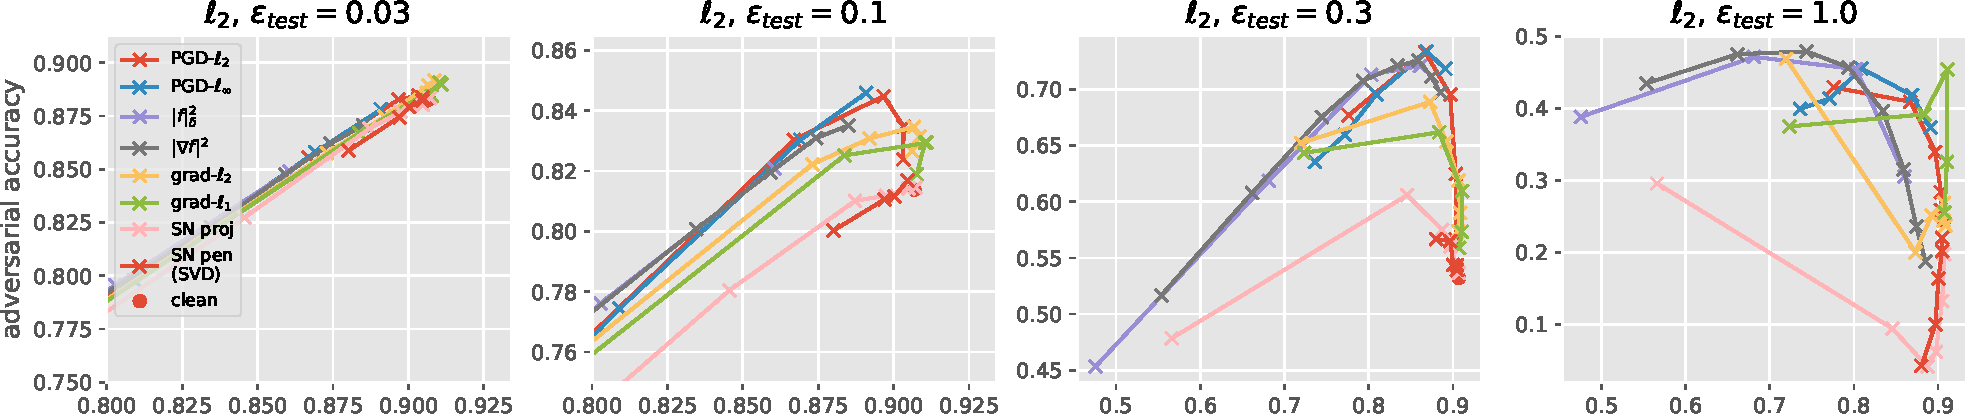
\includegraphics[width=.9\textwidth]{figures/cifar10_vgg/test_vs_adv_l2.pdf}
	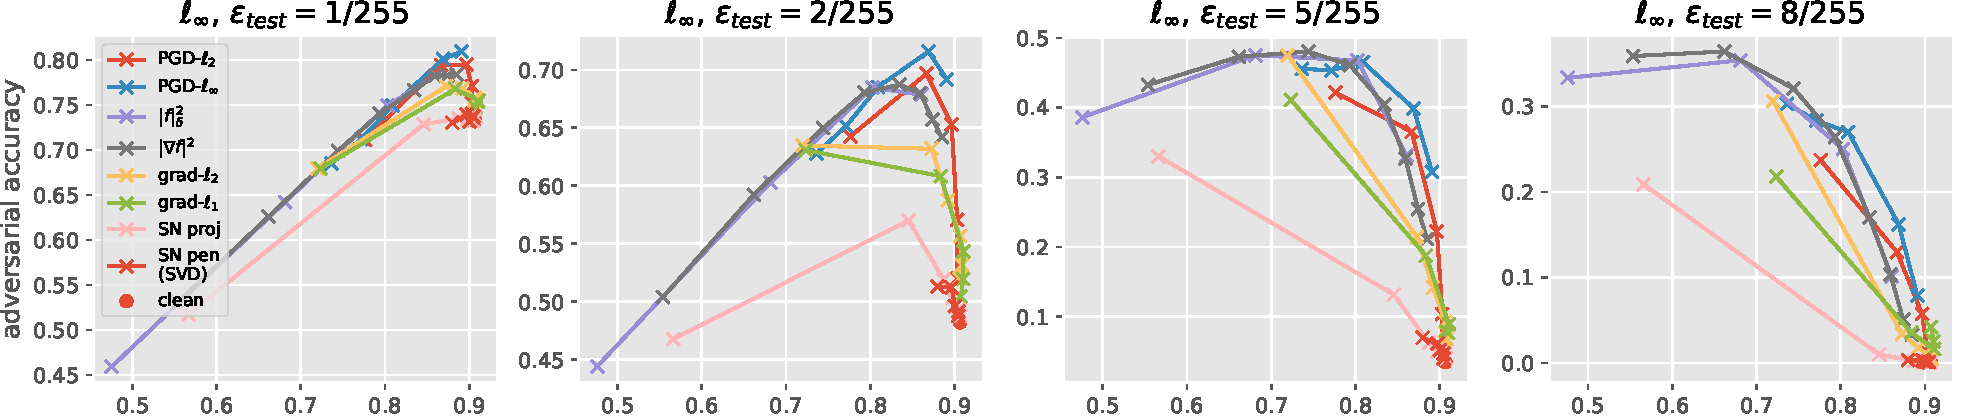
\includegraphics[width=.9\textwidth]{figures/cifar10_vgg/test_vs_adv_linf.pdf}
	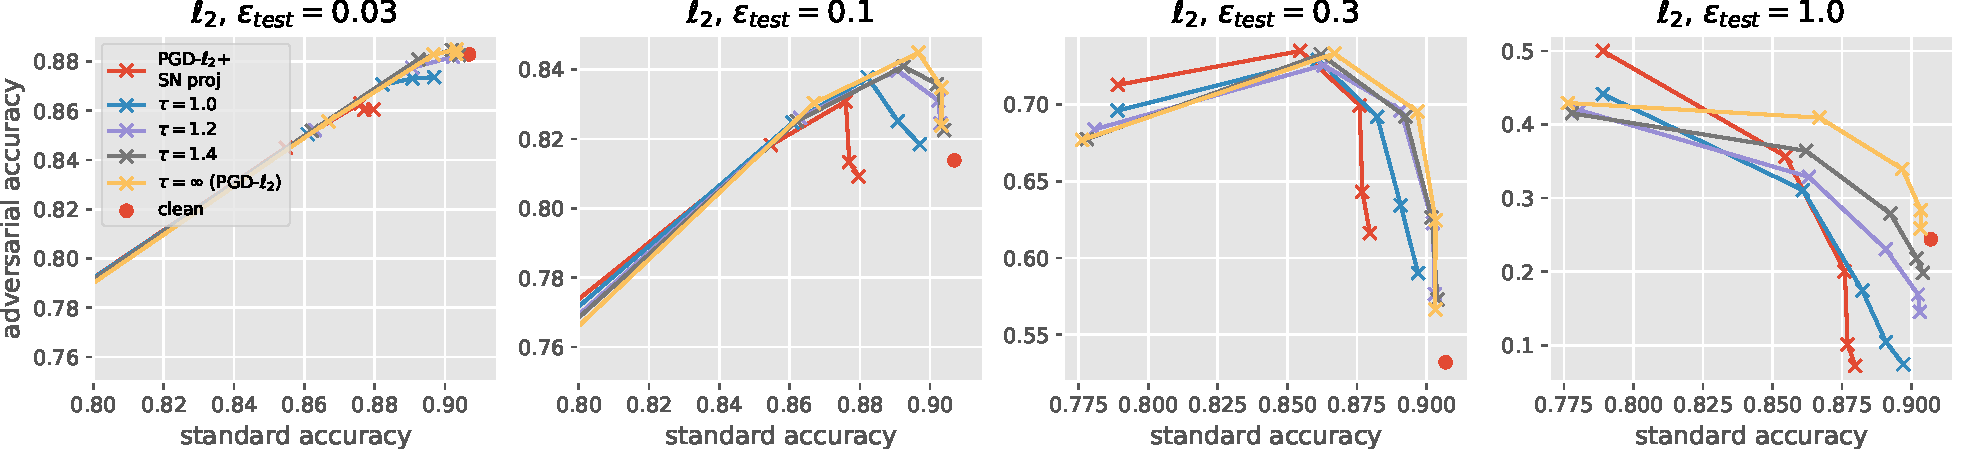
\includegraphics[width=.9\textwidth]{figures/cifar10_vgg/test_vs_adv_comb.pdf}
	\caption{Robustness trade-off curves of different regularization methods for VGG11 on CIFAR10 (extended
	version of Figure~\ref{fig:robust_tradeoffs}).
	The plots show test accuracy vs adversarial test accuracy
	for $\ell_2$-bounded (top/bottom) or $\ell_\infty$-bounded (middle),
	40-step PGD adversaries with a fixed~$\epsilon_{\text{test}}$.
	Different points on a curve correspond to training with different regularization strengths.
	The regularization increases monotonically along a given curve, and
	the leftmost points correspond to the strongest regularization.
	The bottom plots consider PGD-$\ell_2$ + SN projection,
	with different fixed values of the constraint radius~$\tau$, for varying $\epsilon$ in PGD.}
	\label{fig:robust_tradeoffs_appx}
\end{figure*}
